%% LaTeX template for the science justification & technical
%% feasibility to be submitted as part of a Chandra X-ray Observatory
%% proposal.
%%
%% Chandra Cycle 20


%%%%%%%%%%%%%%%%%%%%%%%%%%%
%%%%% DOCUMENT FORMAT %%%%%
%%%%%%%%%%%%%%%%%%%%%%%%%%%

%% The default font was chosen to be easily readable while allowing
%% sufficient material to be included.

%% The two-column, 11pt format fits the largest number of characters
%% per page while still being easily read.

%% There are three documentclass commands provided below. Please
%% uncomment the version you would like to use and comment out the
%% others.

%% Please note that the proposal requires US Letter size pages,
%% 8.5 in x 11 in. PLEASE DO NOT CHANGE THE 'LETTERPAPER' OPTION
%% IN THE DOCUMENTCLASS COMMAND.

%%%%%%%%%%%%%%%%%%%%%%%%%%%%%%%%%%%%%%%%%%%%%%
%%%%% Default format: 11pt single column %%%%%
%%%%%%%%%%%%%%%%%%%%%%%%%%%%%%%%%%%%%%%%%%%%%%

%\documentclass[letterpaper,11pt]{article}

%%%%%%%%%%%%%%%%%%%%%%%%%%%%%%%%%%%%
%%%%% Default font, two-column %%%%%
%%%%%%%%%%%%%%%%%%%%%%%%%%%%%%%%%%%%

\documentclass[letterpaper,11pt,twocolumn]{article}

\usepackage{xspace}

\newcommand{\sun}{$_{\odot}$\xspace}
\DeclareRobustCommand{\ion}[2]{%
\relax\ifmmode
\ifx\testbx\f@series
{\mathbf{#1\,\mathsc{#2}}}\else
{\mathrm{#1\,\mathsc{#2}}}\fi
\else\textup{#1\,{\mdseries\textsc{#2}}}%
\fi}

\def\farcm{\hbox{$.\mkern-4mu^\prime$}}
\def\farcs{\hbox{$.\!\!^{\prime\prime}$}}
\def\degr{\hbox{$^\circ$}}
\def\arcmin{\hbox{$^\prime$}}
\def\arcsec{\hbox{$^{\prime\prime}$}}

\def\aj{AJ}%

          % Astronomical Journal

\def\araa{ARA\&A}%

          % Annual Review of Astron and Astrophys

\def\apj{ApJ}%

          % Astrophysical Journal

\def\apjl{ApJ}%

          % Astrophysical Journal, Letters

\def\apjs{ApJS}%

          % Astrophysical Journal, Supplement

\def\ao{Appl.~Opt.}%

          % Applied Optics

\def\apss{Ap\&SS}%

          % Astrophysics and Space Science

\def\aap{A\&A}%

          % Astronomy and Astrophysics

\def\aapr{A\&A~Rev.}%

          % Astronomy and Astrophysics Reviews

\def\aaps{A\&AS}%

          % Astronomy and Astrophysics, Supplement

\def\azh{AZh}%

          % Astronomicheskii Zhurnal

\def\baas{BAAS}%

          % Bulletin of the AAS

\def\jrasc{JRASC}%

          % Journal of the RAS of Canada

\def\memras{MmRAS}%

          % Memoirs of the RAS

\def\mnras{MNRAS}%

          % Monthly Notices of the RAS

\def\pra{Phys.~Rev.~A}%

          % Physical Review A: General Physics

\def\prb{Phys.~Rev.~B}%

          % Physical Review B: Solid State

\def\prc{Phys.~Rev.~C}%

          % Physical Review C

\def\prd{Phys.~Rev.~D}%

          % Physical Review D

\def\pre{Phys.~Rev.~E}%

          % Physical Review E

\def\prl{Phys.~Rev.~Lett.}%

          % Physical Review Letters

\def\pasp{PASP}%

          % Publications of the ASP

\def\pasj{PASJ}%

          % Publications of the ASJ

\def\qjras{QJRAS}%

          % Quarterly Journal of the RAS

\def\skytel{S\&T}%

          % Sky and Telescope

\def\solphys{Sol.~Phys.}%

          % Solar Physics

\def\sovast{Soviet~Ast.}%

          % Soviet Astronomy

\def\ssr{Space~Sci.~Rev.}%

          % Space Science Reviews

\def\zap{ZAp}%

          % Zeitschrift fuer Astrophysik

\def\nat{Nature}%

          % Nature

\def\iaucirc{IAU~Circ.}%

          % IAU Cirulars

\def\aplett{Astrophys.~Lett.}%

          % Astrophysics Letters

\def\apspr{Astrophys.~Space~Phys.~Res.}%

          % Astrophysics Space Physics Research

\def\bain{Bull.~Astron.~Inst.~Netherlands}%

          % Bulletin Astronomical Institute of the Netherlands

\def\fcp{Fund.~Cosmic~Phys.}%

          % Fundamental Cosmic Physics

\def\gca{Geochim.~Cosmochim.~Acta}%

          % Geochimica Cosmochimica Acta

\def\grl{Geophys.~Res.~Lett.}%

          % Geophysics Research Letters

\def\jcp{J.~Chem.~Phys.}%

          % Journal of Chemical Physics

\def\jgr{J.~Geophys.~Res.}%

          % Journal of Geophysics Research

\def\jqsrt{J.~Quant.~Spec.~Radiat.~Transf.}%

          % Journal of Quantitiative Spectroscopy and Radiative Trasfer

\def\memsai{Mem.~Soc.~Astron.~Italiana}%

          % Mem. Societa Astronomica Italiana

\def\nphysa{Nucl.~Phys.~A}%

          % Nuclear Physics A

\def\physrep{Phys.~Rep.}%

          % Physics Reports

\def\physscr{Phys.~Scr}%

          % Physica Scripta

\def\planss{Planet.~Space~Sci.}%

          % Planetary Space Science

\def\procspie{Proc.~SPIE}%

          % Proceedings of the SPIE

\let\astap=\aap

\let\apjlett=\apjl

\let\apjsupp=\apjs

\let\applopt=\ao

%

\uchyph=0

\usepackage{graphics,graphicx}
% Alter some LaTeX defaults for better treatment of figures:
% See p.105 of "TeX Unbound" for suggested values.
    % See pp. 199-200 of Lamport's "LaTeX" book for details.
    %   General parameters, for ALL pages:
    \renewcommand{\topfraction}{0.9}	% max fraction of floats at top
    \renewcommand{\bottomfraction}{0.8}	% max fraction of floats at bottom
    %   Parameters for TEXT pages (not float pages):
    \setcounter{topnumber}{2}
    \setcounter{bottomnumber}{2}
    \setcounter{totalnumber}{4}     % 2 may work better
    \setcounter{dbltopnumber}{2}    % for 2-column pages
    \renewcommand{\dbltopfraction}{0.7}	% fit big float above 2-col. text
    \renewcommand{\textfraction}{0.07}	% allow minimal text w. figs
    %   Parameters for FLOAT pages (not text pages):
    \renewcommand{\floatpagefraction}{0.7}	% require fuller float pages
	% N.B.: floatpagefraction MUST be less than topfraction !!
    \renewcommand{\dblfloatpagefraction}{0.7}	% require fuller float pages
\def\arcmin{\hbox{$^\prime$}}
	% remember to use [htp] or [htpb] for placement


\usepackage{amssymb}
\usepackage{bibentry,natbib}
\setlength\bibsep{0pt}
\bibliographystyle{prop}

%%%%%%%%%%%%%%%%%%%%%%%%%%%
%%%%% Page dimensions %%%%%
%%%%%%%%%%%%%%%%%%%%%%%%%%%

\setlength{\textwidth}{6.5in} 
\setlength{\textheight}{9in}
\setlength{\topmargin}{-0.0625in} 
\setlength{\oddsidemargin}{0in}
\setlength{\evensidemargin}{0in} 
\setlength{\headheight}{0in}
\setlength{\headsep}{0in} 
\setlength{\hoffset}{0in}
\setlength{\voffset}{0in}



%%%%%%%%%%%%%%%%%%%%%%%%%%%%%%%%%%
%%%%% Section heading format %%%%%
%%%%%%%%%%%%%%%%%%%%%%%%%%%%%%%%%%

\makeatletter
\renewcommand{\section}{\@startsection%
{section}{1}{0mm}{-\baselineskip}%
{0.5\baselineskip}{\normalfont\Large\bfseries}}%
\makeatother



%%%%%%%%%%%%%%%%%%%%%%%%%%%%%
%%%%% Start of document %%%%% 
%%%%%%%%%%%%%%%%%%%%%%%%%%%%%

\begin{document}
\onecolumn
\begin{center} 
\bfseries\uppercase{%
List name, institution and email here if you want to be a Co-I
}
\end{center}
\begin{itemize}
    \item \textbf{PI} Hans Moritz G\"unther, MIT, hgunther@mit.edu
    \item Christian P. Schneider, Hamburg Obervatory, christian.schneider@hs.uni-hamburg.de
\item Gregory J. Herczeg, KIAA/Peking University, gherczeg1@gmail.com
\item Kevin France, University of Colorado, kevin.france@colorado.edu
\item Joel Kastner, Rochester Institute of Technology, jhk@cis.rit.edu
\item Catherine Espaillat, Boston University, cce@bu.edu
\item Connor Robinson, Boston University, connorr@bu.edu
\item L. Ilsedore Cleeves, University of Virginia, lic3f@virginia.edu
\item William J. Fischer, Space Telescope Science Institute, wfischer@stsci.edu
\item Frederick M. Walter, Stony Brook University, frederick.walter@stonybrook.edu
\item David Principe, MIT, principe@mit.edu
\item Nancy Brickhouse, SAO, nbrickhouse@cfa.harvard.edu
\end{itemize}

\twocolumn

\nobibliography{biblio}

\pagestyle{plain}
\pagenumbering{arabic}


 
%%%%%%%%%%%%%%%%%%%%%%%%%%%%%
%%%%% Title of proposal %%%%% 
%%%%%%%%%%%%%%%%%%%%%%%%%%%%%

\begin{center} 
\bfseries\uppercase{%
%%
%% ENTER TITLE OF PROPOSAL BELOW THIS LINE
The power of space: Simultaneous X-ray and UV monitoring of an accreting
low-mass star
%%
%%
}
\end{center}



%%%%%%%%%%%%%%%%%%%%%%%%%%%%%%%%%%%%%%%%%
%%%%% Body of science justification %%%%%
%%%%% and technical feasibility     %%%%%
%%%%%%%%%%%%%%%%%%%%%%%%%%%%%%%%%%%%%%%%%

%%
%% ENTER TEXT AND FIGURES BELOW
%%
Accretion onto low-mass stars can be probed with specific X-ray
signatures observable with Chandra. Observations of the
classical T Tauri star (CTTS) TW Hya indicate that these X-ray
signatures show variability hinting at their accretion origin. We aim
to reveal new accretion physics by observing TW Hya with Chandra/LETGS
simultaneously with already approved HST UV observations in the ULYSSES
program.
%, director's discretionary time program for HST investing about
%1000 HST orbits to observe the UV emission in young stars. ULYSSES
%includes dedicated monitoring observations of TW~Hya, one of the
%closest CTTS. 
The UV and X-ray regimes include tracers of the
accretion process, but it is still unclear how they are related, in
particular since few simultaneous X-ray/UV observations
exist. Existing Chandra grating spectra of TW Hya show variability in emission
lines from the accretion shock on the star. However, the densities in
Ne~{\sc ix} and O~{\sc vii} indicate that today's shock models are
incomplete. A hot wind is the most promising candidate for this
missing component. The HST observations will characterize the wind and
we request five visits of 30 ks Chandra time with LETG/HRC-S
simultaneous to HST to determine the state of accretion. The high
effective area of LETG/HRC-S gives $> 400$ ($>200$) counts in the Ne~{\sc ix} (O~{\sc vii}) triplet in 30~ks, both of which are
crucial for measuring the density and temperature.


\section{Science justification}
Young stars are surrounded by proto-planetary disks, the birthplaces of exo-planets, for the first few Myrs of their existence. Low-mass stars, called classical T~Tauri stars (CTTS) in this phase, accrete mass from the inner rim of the disk. This accretion process produces emission from the NIR to X-rays.

The UV component of this excess emission will be studied by ULLYSES 
\footnote{\url{http://www.stsci.edu/stsci-research/ research-topics-and-programs/ullyses}}
(Ultraviolet Legacy Library of Young Stars as Essential Standards) which is an HST DDT legacy program of  approximately 1,000 orbits with observations from 2020 to 2023. ULLYSES has several components, including 100 orbits dedicated to spectroscopic monitoring of four nearby low-mass stars  starting in the fall of 2020.

We propose Chandra/LETGS observations of TW Hya, the brightest of the four  CTTS that will be monitored by HST/ULLYSES for UV variability.
This will allow us to directly identify physically related phenomena through
their shared variability and to decipher the internal workings of accretion columns.  {\bf Simulatenous X-ray and UV
observations provide an unparalleled opportunity to improve
our understanding of accretion.}


Disk models indicate that X-rays can regulate the chemistry in the disk mid-plane where most of the mass is and planets form (e.g.\ \bibentry{Cleeves_2017}). However, these models are uncertain because because the spatial origin and the time behavior of the X-ray flux and spectrum are not well known.
%% Actually, X-rays may dominate ionization in disk midplanes. Ionization is needed to activate the magneto-rotational instability (MRI) believed to drive viscous accretion (\bibentry{1996ApJ...457..355G}). A very low ionization fraction may suppress the MRI and create a quiescent ``dead zone'' with important implications in planet formation for processes such as dust settling, planetesimal formation, and low mass 
%% planet migration (\bibentry{2007ApJ...654L.159C}; \bibentry{2009ApJ...691.1764M}). 
Therefore
{\bf understanding the high-energy radiation from CTTS is a crucial ingredient to understand the physics and chemistry of star and planet formation.} 

CTTS generate X-ray and FUV emission from active coronae similar to main-sequence stars and from accretion shocks.
The X-ray and UV radiation from the CTTS ionizes parts of the disk and thus the accreting matter follows the stellar magnetic field lines, which connect the star and the disk (e.g. \bibentry{1991ApJ...370L..39K}; \bibentry{1994ApJ...429..781S}). The matter accelerates along the magnetic fields line and hits the stellar surface at free fall velocity.
This accretion shock also heats the surrounding photosphere and veils photospheric lines (\bibentry{Calvet_1998}; \bibentry{2000ApJ...544..927G}). Essentially all methods to derive 
the accretion rate are based on the excess emission caused by the accretion shock. 
%Furthermore, Zeeman-Doppler imaging reveals hot spots with strong magnetic fields, which, in the magnetically funneled accretion model, are the footpoints of the accretion funnels (\bibentry{2007MNRAS.380.1297D}; \bibentry{2008MNRAS.386.1234D}).

Accretion shock models for CTTS predict post-shock plasma
temperatures of 2-3~MK as a result of free-fall velocities of 
300-500\,km\,s$^{-1}$. Such a shock cools predominately by
X-ray emission, which is partly reprocessed into UV emission within the regions surrounding the shock (see Fig.~\ref{fig:CIVsketch}, left). 

\begin{figure*}
\centering
\resizebox{\hsize}{!}{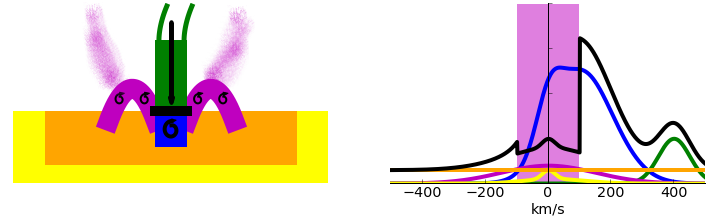
\includegraphics{figs/sketch3_modified}}
\caption{\label{fig:CIVsketch} \emph{left:} Structure of the accretion
  shock in low-mass stars. Indicated are the pre-shock (green) and
  post-shock (blue) gas, which heats some of the photosphere (yellow
  and orange where heated). The post-shock gas is responsible for the
  X-ray emission. The megenta material is an up-spill or outflow,
  which will be probed by the UV observations.  
  \emph{right:}
  Working hypothesis for the observed UV lines profiles.
  Individual contributions to the line profile (color) and total line
  profile (black). 
  % The yellow line (photosphere) shows the C~{\sc iv} in a
  % young, non-accreting star; 
  The pre-shock gas (green) emits close
  to the free-fall velocity. Post-shock gas (blue) emits
  between 0 and 125~km/s with turbulent broadening. The
  spilled up gas (magenta) escapes the funnel. Due to turbulence and bulk
  motion it causes a very wide line. It also blocks the view of
  the accretion column. 
  %The heated photosphere (orange)
  %can be described by a black-body
  %continuum.
  }
\end{figure*}


\underline{\bf X-rays}: The observability of the ``primary'' X-ray photons 
escaping the post-shock region is still debated 
(\bibentry{Guenther_2007}; \bibentry{Argiroffi_2009}; \bibentry{Sacco_2010}). Observationally, 
however, accreting (low-mass) stars show  an excess of plasma with 2-3~MK
compared to main-sequence stars (\bibentry{Robrade_2006}; \bibentry{Guedel_2007}).
On the other hand, the measured X-ray line fluxes typically fall short of
predictions from quantitative shock models for the accretion rates derived with non-X-ray tracers (\bibentry{Curran_2011}). TW~Hya is the only known example where all accretion tracers are reasonably consistent with each other (\bibentry{Brickhouse_2010}). 


\underline{\bf UV ion lines}:  Deriving  accretion rates from UV line fluxes is based 
on flux-flux scaling relations, not on quantitative shock models. Where those models make predictions, they sometimes disagree with observations. For instance, it is believed that the  narrow and 
broad components of the C~{\sc iv} lines  originate in the post- and 
pre-shock material, respectively (\bibentry{Ardila_2013}). However, only a few systems show the
expected ratio between the pre- and post-shock velocities and line
shifts are generally too low compared to free-fall velocities. 

\underline{\bf UV continuum}: The FUV continuum emission in CTTS is
dominated by the hot spot in the photosphere, which is heated up by
reprocessing the energy deposited in the accretion shock. In
TW Hya HST/COS monitoring shows the FUV
continuum to vary by a factor of three on time scales of days
(Fig.~\ref{fig:UV2}) presumably due to variations in the
accretion rate and viewing geometry. There is similar variability in
GM~Aur, also one of the ULLYSSES targets (\bibentry{Robinson_2019}).

%\underline{\bf UV H$_2$ emission}: FUV spectra of CTTS show a large number of ro-vibrational H$_2$ emission lines which are formed in the upper layer of the disk out to a disk radius of several au. They are excited by the Ly$\alpha$ emission from the infalling column and the accretion shock (\bibentry{2004ApJ...607..369H}; \bibentry{2017ApJ...844..169F}). 

{\bf Neither the X-ray nor the UV accretion signatures are fully explained by existing models}. Still, we expect the following X-ray vs.\ UV correlations and time scales if our current picture is roughly correct:
\begin{enumerate}
    \itemsep1pt
    \item Soft X-ray flux from the shock and UV ion lines from the shock should be correlated on the shock-crossing time scale (minutes).
    \item Shock densities measured from X-ray grating
      spectroscopy and UV continuum from the
      photosphere heated by the shock should be correlated on time
      scales of hours.
    \item Large X-ray flares cause a reconfiguration of the stellar
      magnetic field. This will change which field lines connect to
      the disk and how much mass they carry (free-fall time scale:
      hours). The latter is observed in UV ion lines and continuum.
    %\item We expect a relation between soft X-ray flux and UV Ly$\alpha$ from the shock on the one side and the UV H$_2$ emission from the irradiated disk over a sample with different disk properties and accretion rates.
\end{enumerate}

\textbf{A monitoring program with simultaneous, or at least contemporaneous, X-ray and UV spectroscopy
is needed to unambiguously identify how the different 
accretion tracers are physically related.} The proposed joint X-ray and UV observations are ideally
suited to utilize the intrinsic accretion variability in
CTTS to better understand the physics of accretion and to move beyond 
empirical flux-flux calibrations. 

Monitoring has been previously attempted in TW Hya. In 2011 we obtained Chandra DDT
data with LETGS/ACIS (at the time, the ACIS contamination was much lower than
today), within one hour of HST/COS data.
We tried again in March of 2019 with HETG/HRC-I. This 70~ks exposure was split into two
observations, two days apart. The second one was supposed to be taken simultaneous to HST data,
but a Chandra command error caused that exposure to fail. It was
re-scheduled about three month later. Incidentally, the HST observations
suffered from an acquisition error and were also re-scheduled, but despite the
best efforts of the Chandra and HST scheduling teams, the time difference
between the HST and Chandra data is two days - longer than the time scale of the
UV variability as shown in Fig.~\ref{fig:UV2}. \textbf{Unfortunately, that
  means we have only one 20~ks X-ray grating observation that is separated by
  $<1$ day from UV spectroscopy.}

\begin{figure}
\begin{center}
\resizebox{1\hsize}{!}{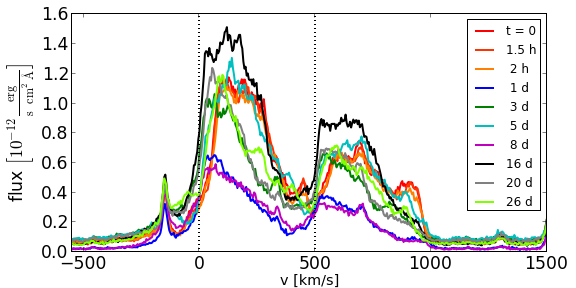
\includegraphics{figs/CIV}}
\end{center}
\caption{\label{fig:UV2} C~{\sc iv} lines in TW Hya with HST/COS in a setup that will also be used in the ULLYSES observations. The legend lists for each spectrum how long after the
  start of the campaign this data was observed. The dotted lines mark the rest wavelengths of the two
  lines in the \ion{C}{iv} doublet. The narrow emission feature at $-125$~km/s is
  an unrelated $H_2$ line. The change in continuum is real. The line profiles vary widely. \textbf{Note that the three
profiles taken in consecutive orbits are very similar, but even 1~day later,
the line profile is markedly different.} The two spectra where both line and
continuum are faint, are observed 7 days apart with different states of the
emission lines in between.}
\end{figure}


We know that both X-ray and UV properties change over time, the UV in
quite dramatic fashion (Fig.~\ref{fig:UV2}), the X-rays more
subtle. In Fig.~\ref{fig:allspec} we show a powerful diagnostic
(\bibentry{2012ApJ...760L..21B}) that is enabled by the Chandra
gratings. We determine the temperature of the Ne~{\sc
  ix} emitting gas from the temperature sensitive G-ratio in the He-like triplet around 13.5~\AA{} ($(f+i)/r$ line ratio) and
compare that to the ratio He$\alpha$/He$\beta$ of the same ion
(y-axis). Since the He$\alpha$ and He$\beta$ lines are separated more
in the spectrum than the triplet lines, a comparison between observed
and predicted ratios reveals the absorbing column
density. \textbf{Using an accretion model, \citet{2012ApJ...760L..21B}
  show that the apparently subtle changes in the X-ray grating
  spectrum require very significant changes (factor of a few,
  Fig.~\ref{fig:Brickhouse_3}) in accretion rate, filling factor, and
  polar magnetic field strengths. }

\begin{figure}[h!]
\centering
\resizebox{\hsize}{!}{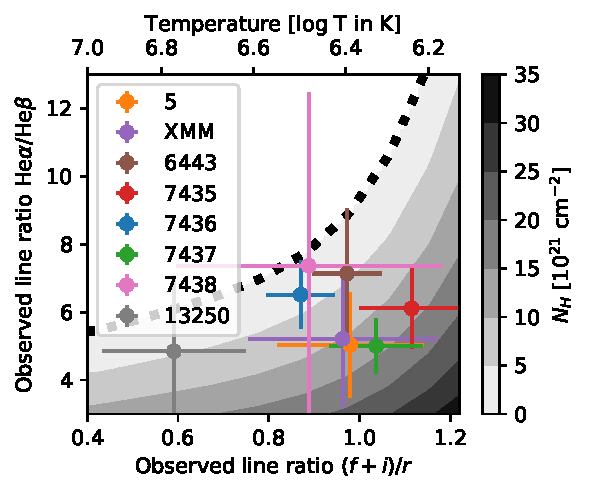
\includegraphics{figs/Ne-var}}
\caption{Ratio of the flux of the resonance line (He$\alpha$, also
  called ``r'') to that of He$\beta$ compared to the observed
  $(f+i)/r$ ratio for Ne~{\sc ix}. Both ratios are temperature
  sensitive (top axes gives temperature derived from $(f+i)/R$
  ratio). Without absorption, datapoints points would lie on the
  dotted line.  Many of the observations require significant
  absorption of the Ne~{\sc ix} emission. Chandra ObsIDs are labelled.
\label{fig:allspec} }
\end{figure}


\begin{figure}[h!]
\centering
\resizebox{\hsize}{!}{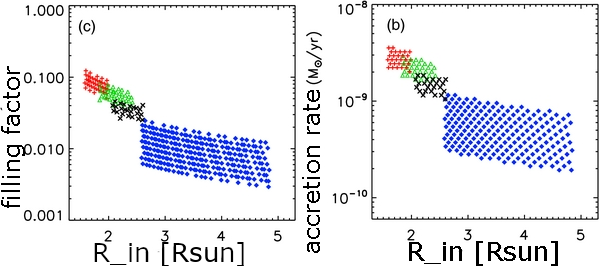
\includegraphics{figs/Brickhouse12_fig3}}
\caption{Seemingly small changes in measured line ratios can have big
  implications for the physical parameters. The plot shows how the
  area covered in spots (filling factor) and mass accretion rate
  differ by a factor of a few between the observations marked red,
  green, and blue in Fig.~\ref{fig:allspec}. Symbols are models from a
  grid compatible with observed ratios within the errors. X-axis shows
  inner radius of accretion disk. Modified from:
  \protect{\citet{2012ApJ...760L..21B}}
\label{fig:Brickhouse_3} }
\end{figure}



\section{Immediate objective}
We can see in Fig.~\ref{fig:UV2} that UV continuum and line emission varies dramatically, there might even be two distinct states (Fig.~\ref{fig:CIVsketch}). We want to link the UV state to an X-ray state to get a complete picture of accretion. In X-rays we always observe f/i ratios lower than those of typical coronal densities which are thus presumed to come from an accretion shock. Yet, in the UV, the continuum and the hot ion line emission varies widely. Why is that? Can we link the visibility of the UV continuum and the C~{\sc iv} line to $N_H$ variations in the X-rays, i.e.\ is some of the shock buried? Or is this a change in the structure of the shock, i.e.\ do we see changes in the UV line profiles because the infall speed changes? In that case, UV variability would correlate with X-ray temperature changes.
To distinguish between these possibilities, \textbf{we need X-ray grating spectroscopy contemporaneous to already approved HST DD observations of TW Hya.}






\section{Feasibility}
%The effective area at the location of the Ne~{\sc ix} triplet for HETG/ACIS-S in 2007 (when the data used in
%\citet{2012ApJ...760L..21B} was taken) is about 20\% larger than LETG/HRC-S
%today. (HETG/ACIS-S effective area is reduced by about a factor of 5 today
%compared to 2007 because of the ACIS contamination.)
We need X-ray grating observations within 6~h of the UV data (see UV
variability in Fig.~\ref{fig:UV2}). The ULLYSES UV observations will
be distributed as follows (private communication with the ULLYSES team
at STScI): Four observations per rotation period for three consecutive
periods. For TW~Hya that means that HST observations will be separated
by about one day for twelve days. This covers about five Chandra
orbits. Given current thermal constraints, Chandra can observe TW~Hya
typically once per orbit and the thermal time scale for Chandra is
about 30~ks. Thus, we request five observations of 30~ks each. The
high effective area of LETGS/HRC-S gives $> 400$ ($>200$) counts in
the Ne~{\sc ix} (O~{\sc vii}) triplet, both of which are crucial for
measuring the density and temperature.  In Fig.~\ref{fig:allspec} the
error bars for each 30~ks segment will be about 2.2 times larger than
ObsID~6443 which uses the same setup. If segements are split further
or the error bars from individual segments in a figure like
Fig.~\ref{fig:allspec} overlap, we can combine segments that show
similar UV properties in the quasi-simultaneous HST observations.
\textbf{Only grating data can reveal density, temperature, and
  absorption of the accretion shock.}  In CCD data, lines are not
resolved, and shock and coronal contribution cannot be
separated. Nevertheless, the interpretation will be helped by our
already approved NICER observations, which will be scheduled to catch
the HST orbits missed by Chandra to provide a multi-band X-ray
lightcurve.
 
%% Technical Justification for Joint Facilities section
%% comment this section out on proposals not asking for
%% joint time

%\section{Technical Justification for Joint Facilities}



%% References section

%\section{References}


%%%%%%%%%%%%%%%%%%%%%%%%%%%
%%%%% End of document %%%%%
%%%%%%%%%%%%%%%%%%%%%%%%%%%
%\bibliography{biblio}

\end{document}
